\documentclass[conference]{IEEEtran}
\usepackage{graphicx} % Required for inserting images
\usepackage{float}
\usepackage{subcaption}

\def\BibTeX{{\rm B\kern-.05em{\sc i\kern-.025em b}\kern-.08em
    T\kern-.1667em\lower.7ex\hbox{E}\kern-.125emX}}
\begin{document}

\title{Data Mining Project: Analyzing Video Game Sales\\
{\footnotesize \textsuperscript{*} CS 4412: Data Mining}

}

\author{\IEEEauthorblockN{Joshua Vach}
\IEEEauthorblockA{\textit{Student at Kennesaw State University} \\
Marietta GA \\
jvach3@students.kennesaw.edu}

}
\maketitle
\section{Data Preprocessing and Transformation}
While the data contained in the video game csv database is mostly full and accurate there are a few missing values mainly in years which has several games without years labeled as NA which is simple to deal with pandas dropna command. There are also several games within the dataset that have 0 sales in certain sales markets this however is not a problem as they have data stored there it is just 0. For data pertaining to years there is one outlier in this dataset that released in 2020 with the other latest being in 2017 so for calculations relating to years of release it must be removed. 

To answer our first discovery question we created 3 percentages for every data point that showed the percentage of global sales in each major market (JP, EU, NA) and then used these to run our K means to group points using these 3 percentages and year of release.

Our second discovery question was focusing on platform sales compared to its highest earner so we found the total sales for every platform as well as the highest selling game on that platform in that year, and made a ratio of how much of the total sales were made by the highest selling game that year. This was then used alongside total sales per platform to group the platforms together. 

To answer the third question was more difficult but similar to the answering for the first question, but instead of being total for the game it sums the total sales per year for the major markets(JP, EU, NA) and compare it to the global total sales that year. This is then used to group the data alongside total sales and year using k-means.
\section{Exploratory Data Analysis}
We did several exploratory data in order to find out a baseline for trends happening in the game industry over time.
\subsection{Video Game Releases per Year}
The first data analysis is the amount of games released per year to show the growth of the games industry over time.


\begin{figure}[H]
    \centering
    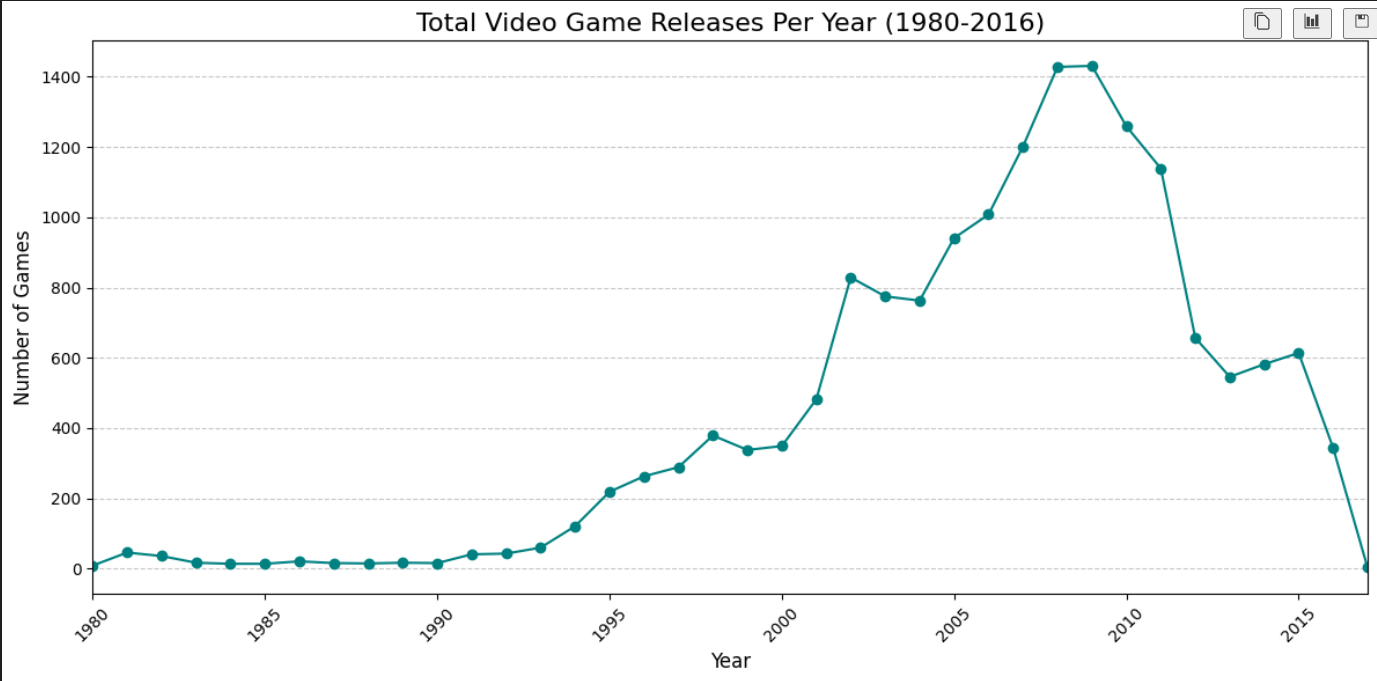
\includegraphics[width=0.8\linewidth]{vgreleases.png}
    \label{fig:placeholder}
\end{figure}

\subsection{Top Publishers, Genre, and Platform by releases}
We analyzed several different data points in the dataset in order to find the top genre publishers and platform in  order to find broad trends based on this data. We found that the DS and PS2 were dominant in the platform department and EA is dominant in the publishing department while Action and Sports are the two largest genres by a wide margin.
\begin{figure}[H]
    \centering
    \begin{subfigure}[b]{0.2\textwidth}
        \centering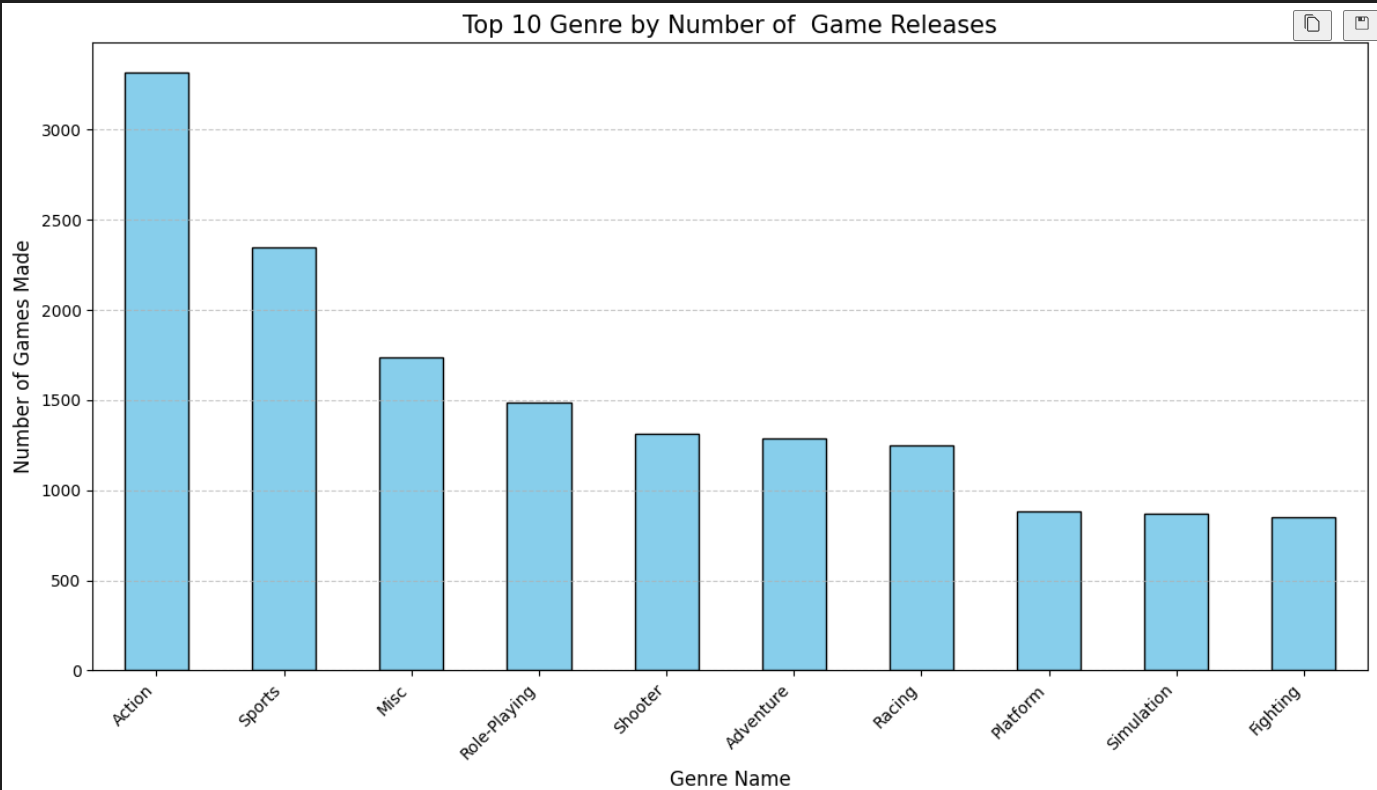
\includegraphics[width=\textwidth]{vggenre.png}
    \end{subfigure}
    \hfill
    \begin{subfigure}[b]{0.2\textwidth}
        \centering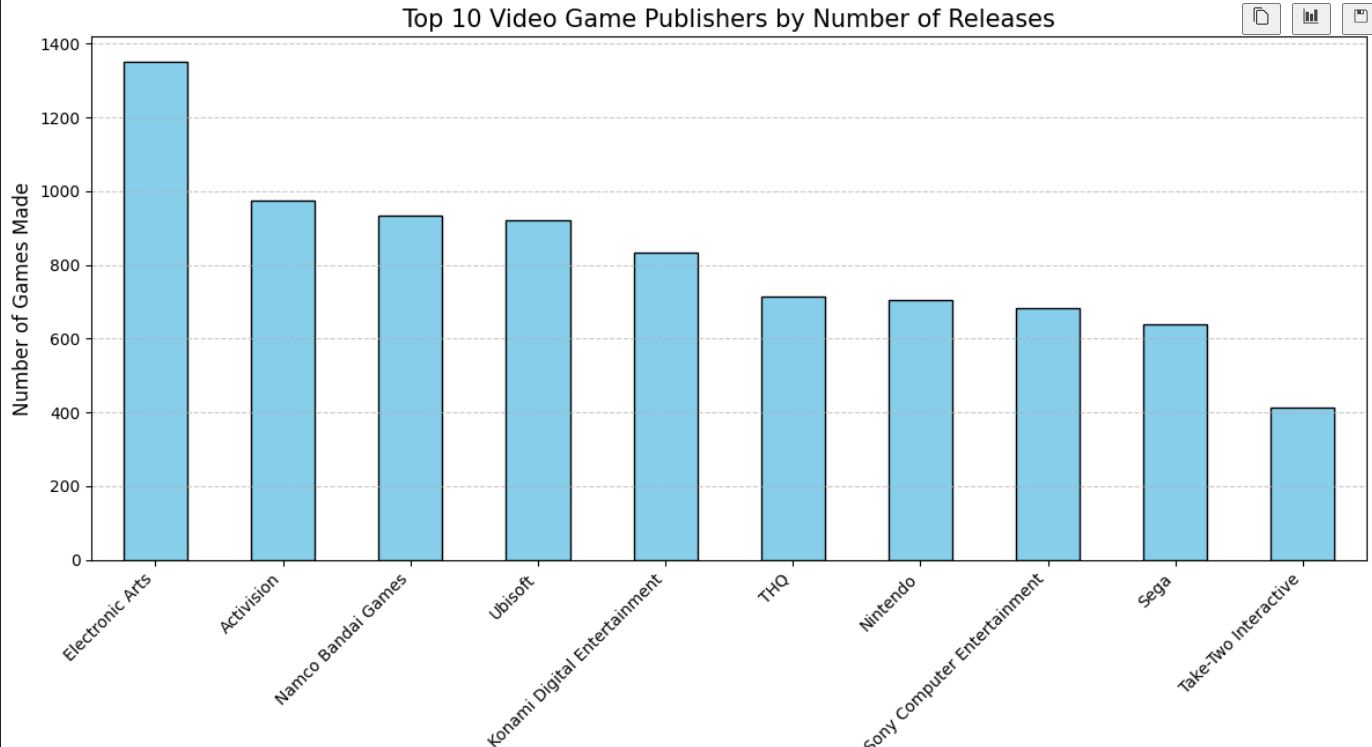
\includegraphics[width=\textwidth]{vgpublish.png}
    \end{subfigure}
    \hfill
    \begin{subfigure}[b]{0.2\textwidth}
        \centering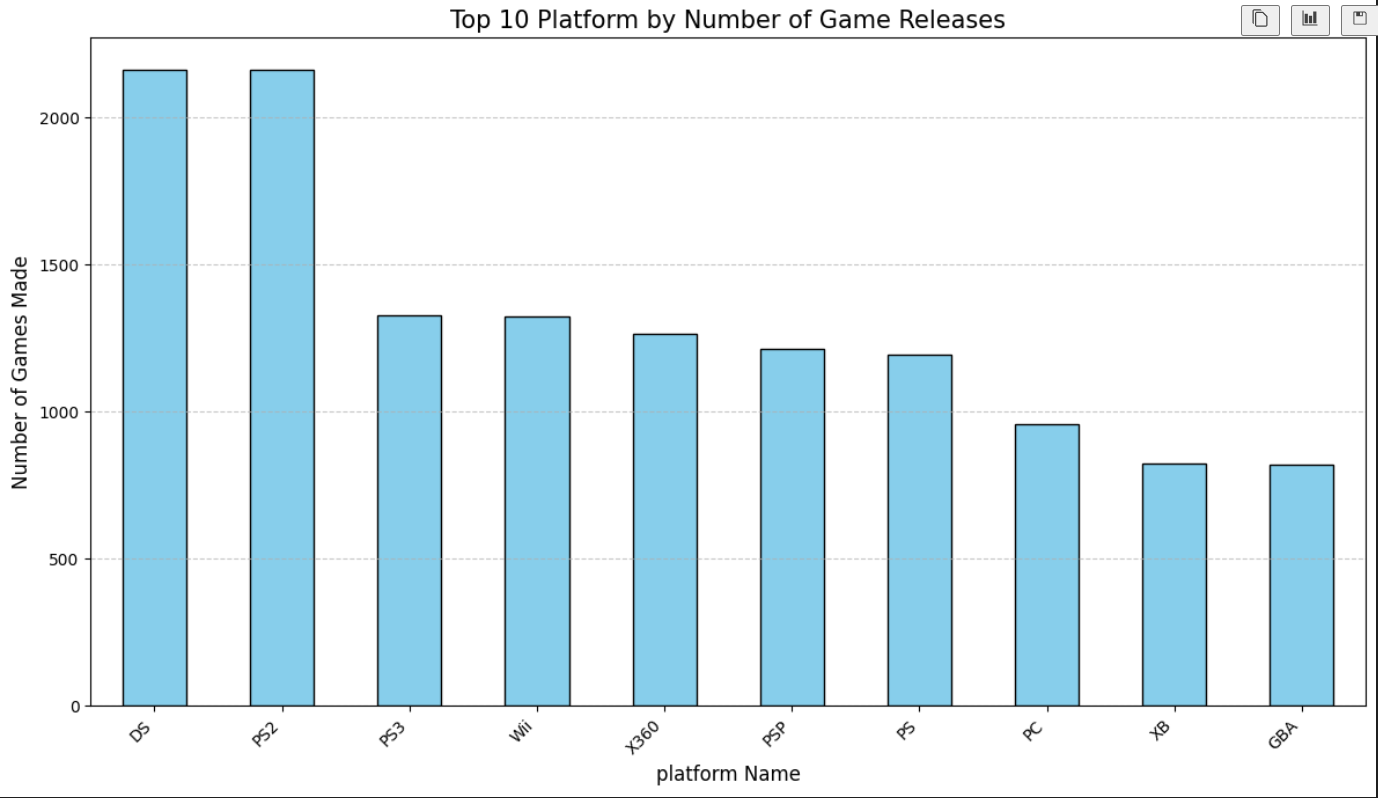
\includegraphics[width=\textwidth]{vgsalesplat.png}
    \end{subfigure}
\end{figure}


\subsection{Sales Trend by Region}
We also analyzed the total sales both globally and in the major markets in order to get an overview of how sales have changed in the various markets over time.

\begin{figure}[H]
    \centering
    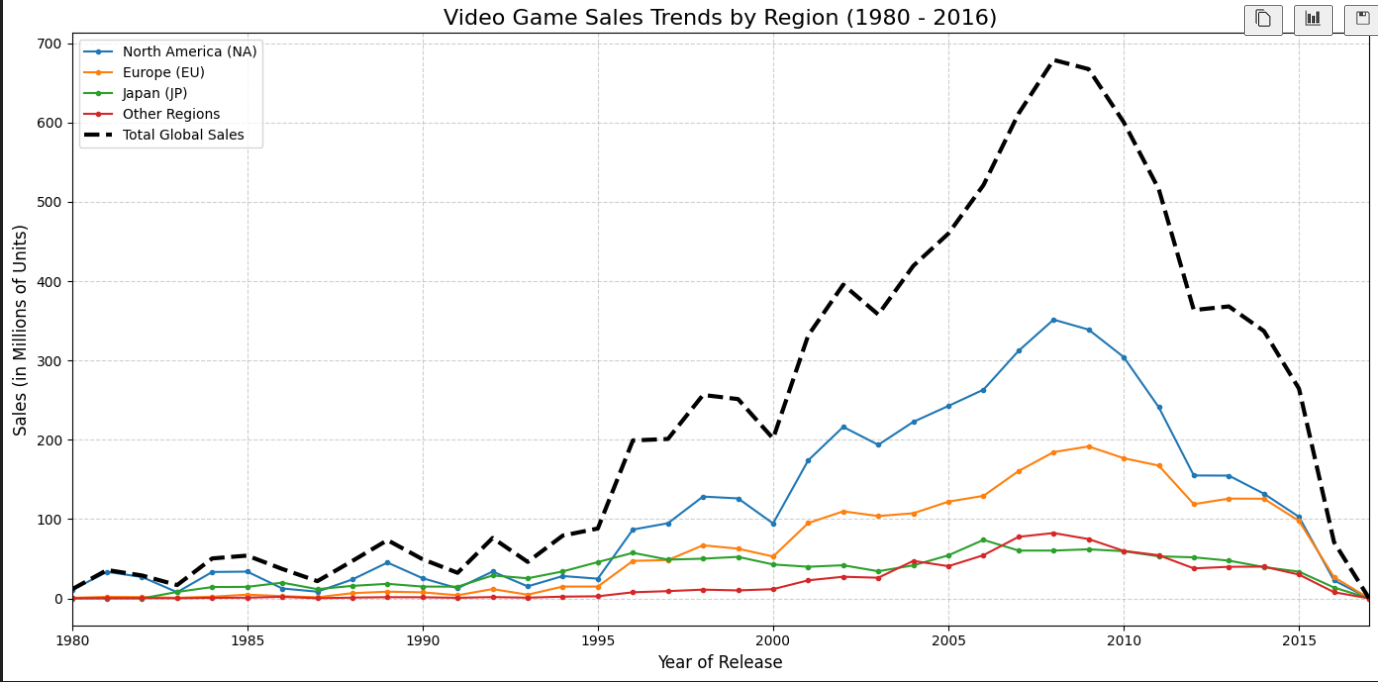
\includegraphics[width=0.8\linewidth]{vgsalesregion.png}
    \label{fig:placeholder}
\end{figure}

\subsection{Sales Comparison by Region for Publishers and Platforms}
In order to properly analyze how each platform and publisher does in every market to see if the home market of the publisher/platform has any effect on its performance in other markets
\begin{figure}[H]
    \centering
    \begin{subfigure}[b]{0.2\textwidth}
        \centering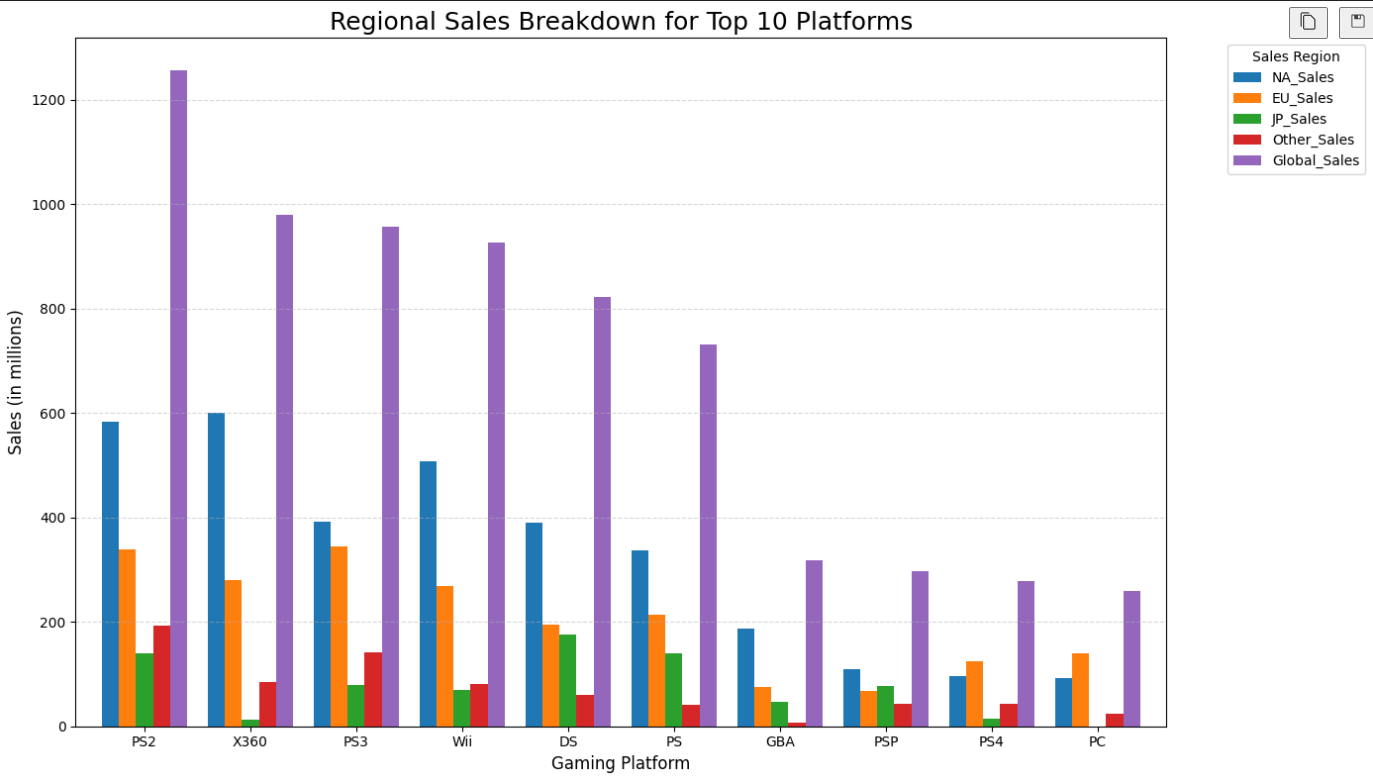
\includegraphics[width=\textwidth]{vgsalesplatform.png}
    \end{subfigure}
    \hfill
    \begin{subfigure}[b]{0.2\textwidth}
        \centering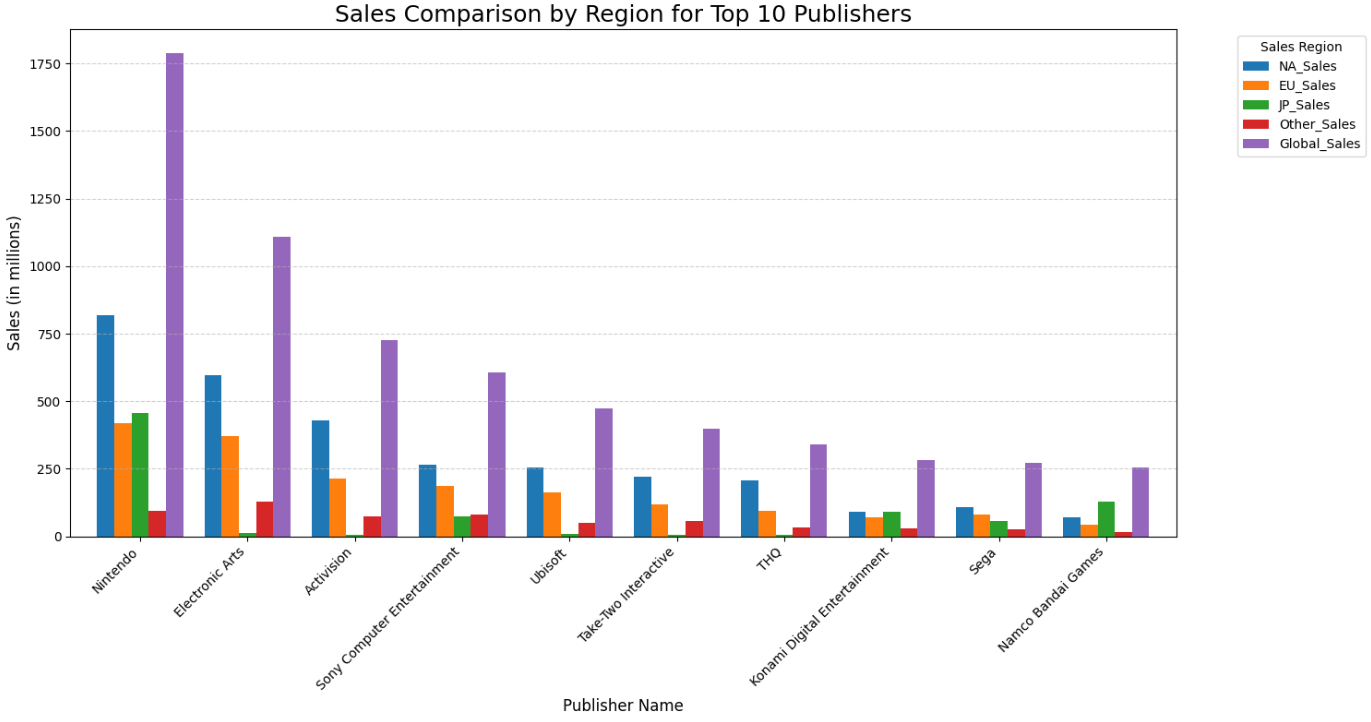
\includegraphics[width=\textwidth]{vgsalespublisher.png}
    \end{subfigure}
\end{figure}

\subsection{Sales Comparison of top 10 Platforms and Publisher over time}
Tracking and Analyzing how sales of various publishers and platforms perform over time can show changes in consumer sentiment as well as show which publishers do better when each platform is most popular. Nintendo dominates with sales especially during the era where the Wii was the most popular console.

\begin{figure}[H]
    \centering
    \begin{subfigure}[b]{0.2\textwidth}
        \centering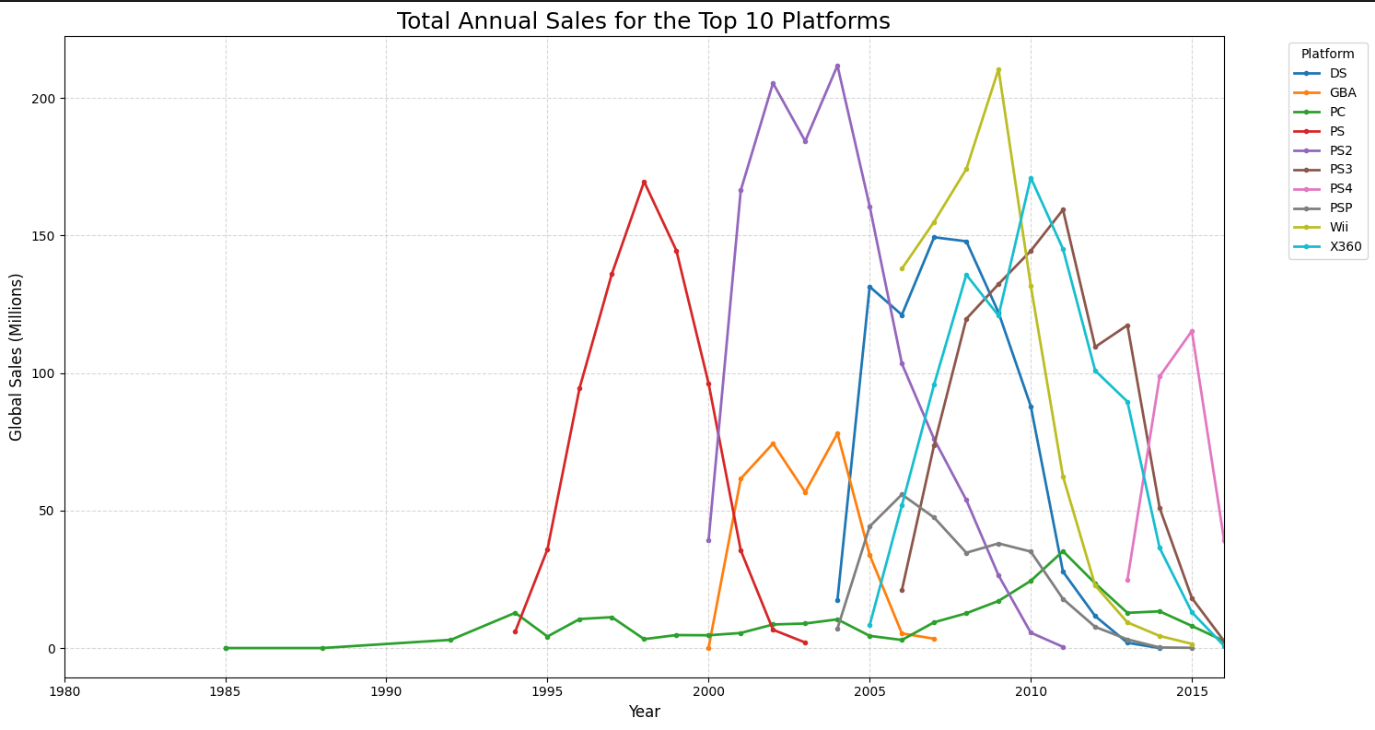
\includegraphics[width=\textwidth]{vgsalesplatovertime.png}
    \end{subfigure}
    \hfill
    \begin{subfigure}[b]{0.2\textwidth}
        \centering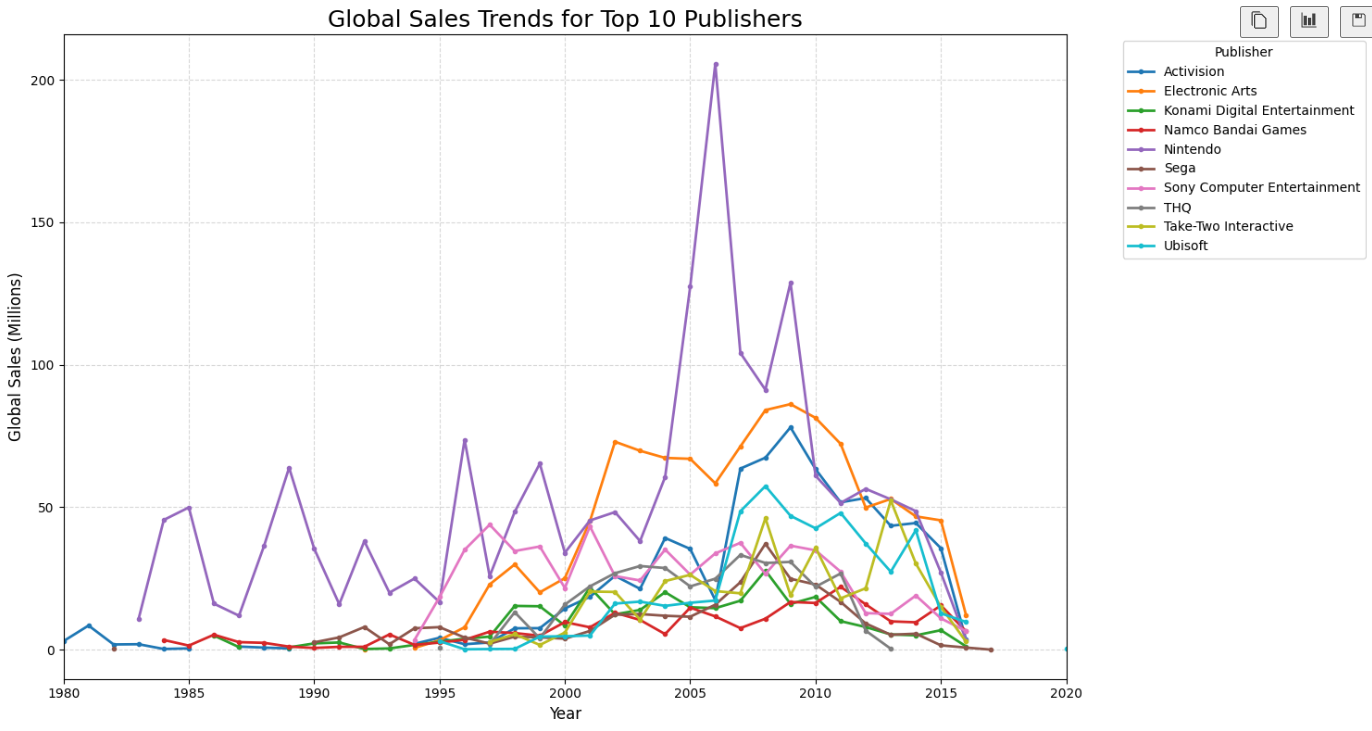
\includegraphics[width=\textwidth]{vgsalespubtime.png}
    \end{subfigure}
\end{figure}

\section{K-means Analysis}
In this deliverable, we used K-means to analyze the dataset to attempt to answer our 3 discovery questions.
\subsection{Question 1: Market Success in Home Market Against Foreign Market}
In addition to the sales, we analyze the characteristics of the clusters including average sales percentage in each market and year, as well as the top 3 consoles in each cluster.
\begin{figure}[H]
    \centering
    \begin{subfigure}[b]{0.2\textwidth}
        \centering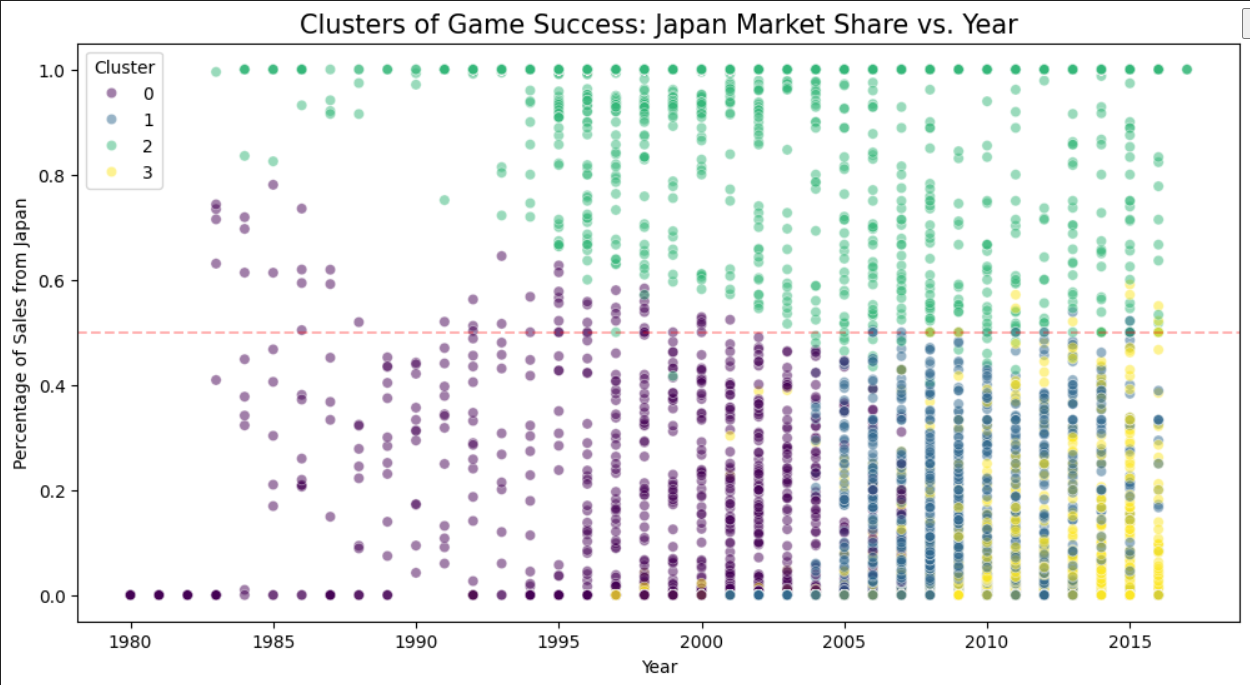
\includegraphics[width=\textwidth]{kmeasnques1.1.png}
    \end{subfigure}
    \hfill
    \begin{subfigure}[b]{0.2\textwidth}
        \centering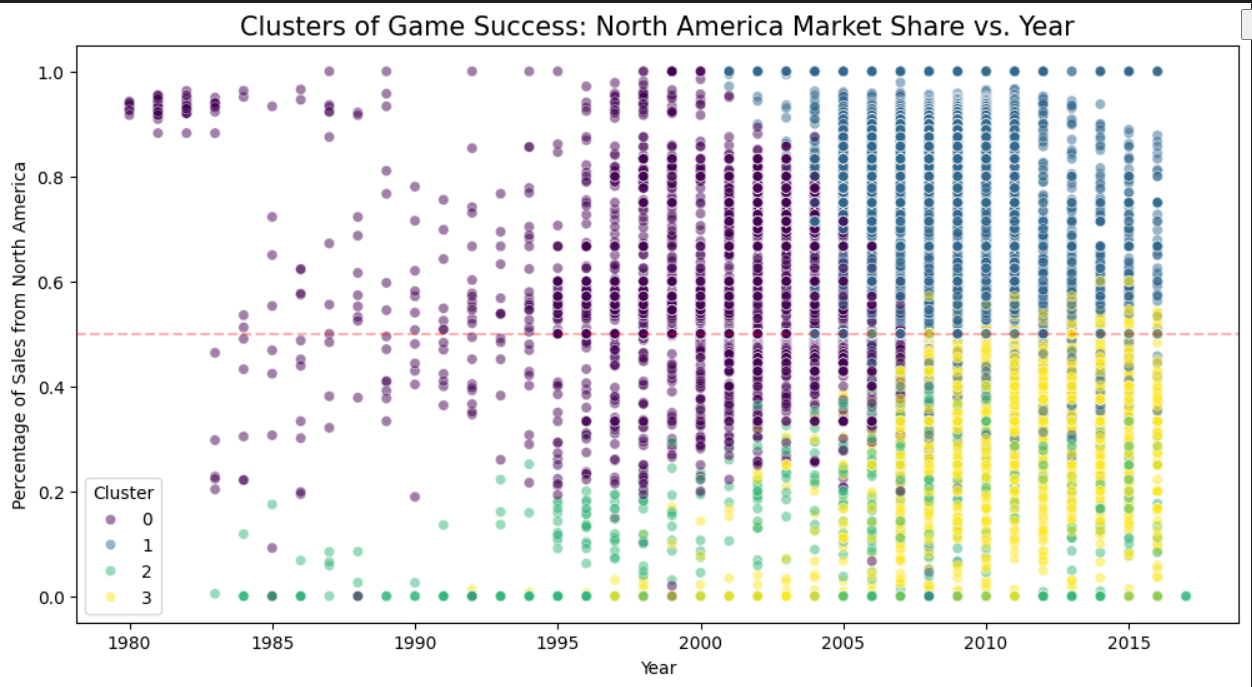
\includegraphics[width=\textwidth]{kmeansques1.2.png}
    \end{subfigure}
    \hfill
    \begin{subfigure}[b]{0.2\textwidth}
        \centering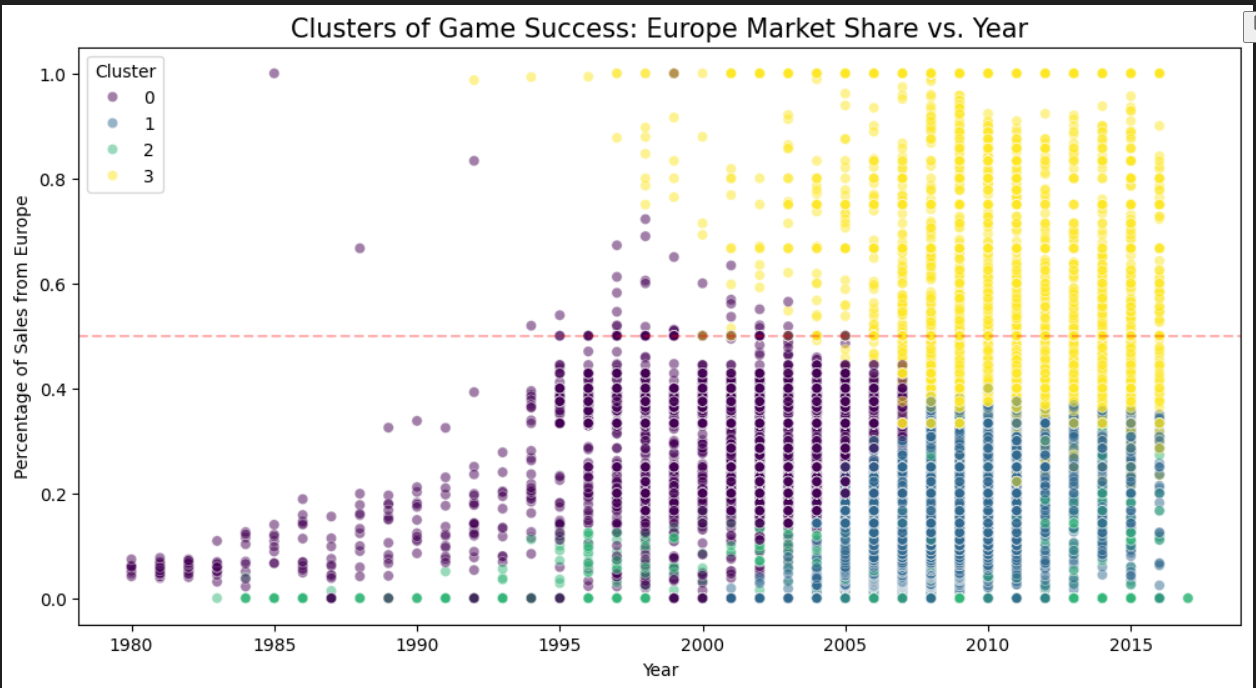
\includegraphics[width=\textwidth]{kmeansques1.3.png}
    \end{subfigure}
\end{figure}
Cluster 2 shows that there are  a lot of Japanese games that do not make it outside of Japan. Other clusters are more mixed but 2 is overwhelmingly dominated by Japan. Cluster 0 and 1 are both dominated by North American sales but have average years of 2000 and 2008 respectively. Cluster 3 is a European centered cluster while also having the highest average year which shows Europeans have moved into the market more recently compared to the other markets. Cluster 0 and 1 both have highest platforms being mainly of Japanese origin with 0 having PS2 PS and GBA and 1 having DS Wii and xbox 360. this shows that while the Japanese game companies still dominated the later game industry North American companies began to move into the market later on. One interesting note is that in cluster 3 PC was the largest platform which shows that PC games typically sell well in Europe but not as well in other markets.
\subsection{Question 2: Finding Healthy Platform Ecosystems and Platforms Dominated by Single Games}
\begin{figure}[H]
    \centering
    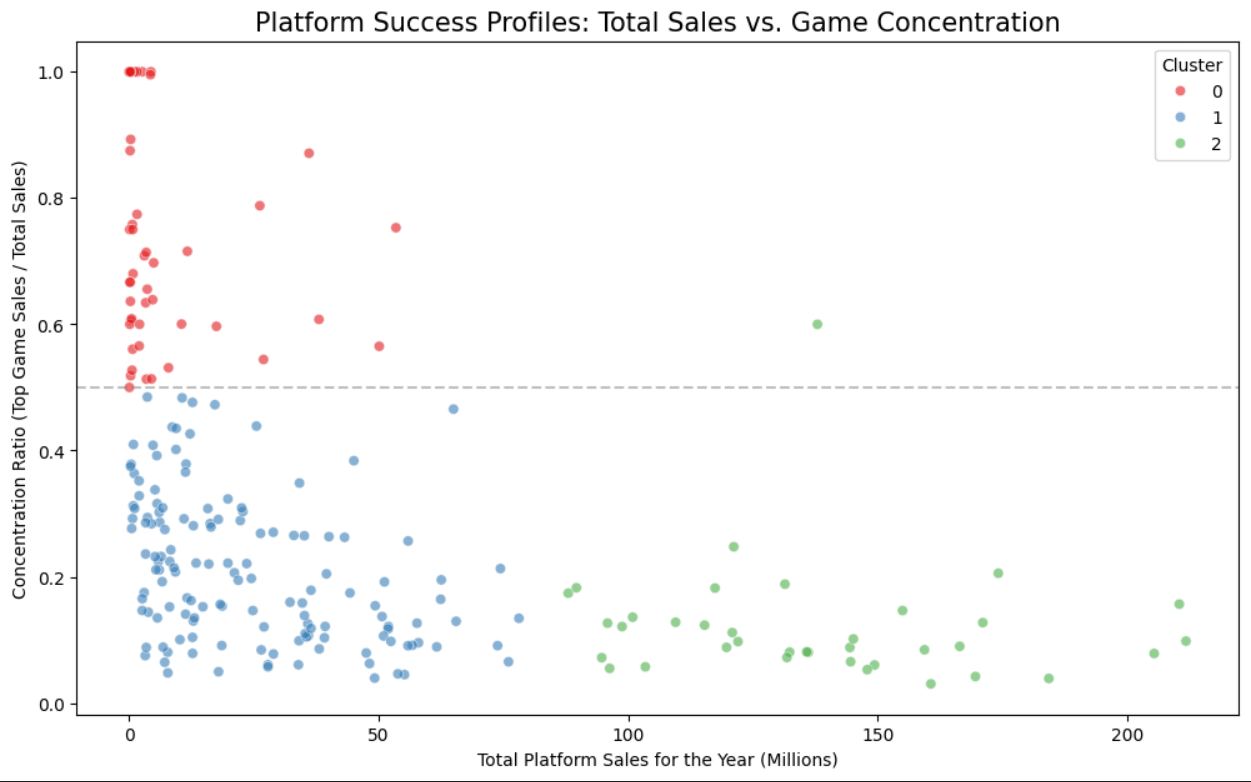
\includegraphics[width=0.8\linewidth]{kmeansques2.png}
    \label{fig:placeholder}
\end{figure}
This analysis has lead to several interesting observations with the 3 clusters. Cluster 0 are platforms that sold poorly that year and only really had one game that pushed its sales up, cluster 1 is platforms that sold poorly that year and had a multitude of games making up its low sales. Cluster 2 is made up of well performing consoles that sold well with lots of games making up the sales. There is one outlier in this cluster though that sold almost 150 million copies with one game making over 60 percent of those sales. This is most likely the best selling game, Wii sports, making up most Wii sales that year
\subsection{Question 3: Change in Market share Over Time}
\begin{figure}[H]
    \centering
    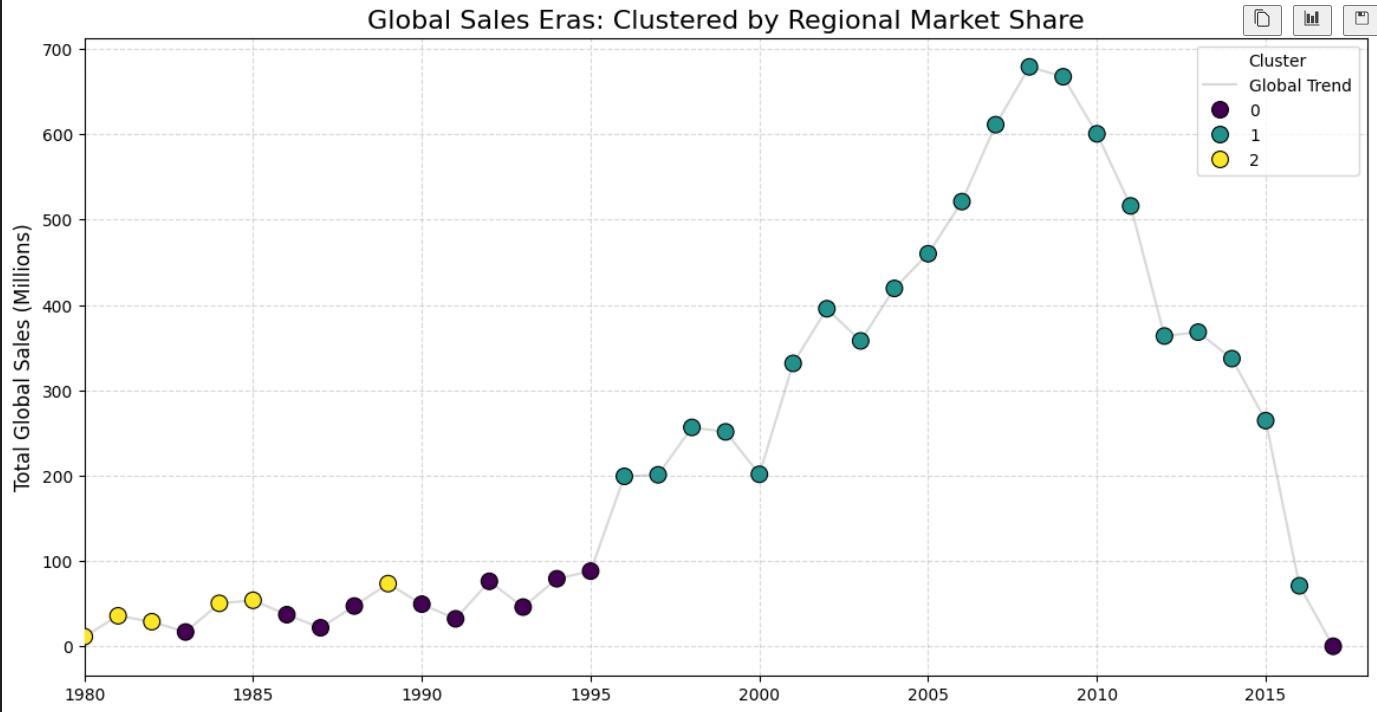
\includegraphics[width=0.8\linewidth]{kmeansques3.png}
    \label{fig:placeholder}
\end{figure}
This analysis was the least insightful of the 3 K-means analysis. There were 3 clusters. Cluster 0 consisted of mainly Japanese sales and shows an era of Japan holding most of the video game market at the start. Cluster 1 is the modern global era of video game sales with high sales all over the world but mainly in North America.  Cluster 2 is dominated by North America with 78 percent of sales being from North America. Cluster 2 has an outlier in 2017 due to the low amount of data in that year. This data shows a shift during the 90's away from Japan as a dominant force in gaming towards North America and finally towards a global market.
\end{document}




